\documentclass[sigchi-a, authorversion]{acmart}
\usepackage{booktabs} % For formal tables
\usepackage{ccicons}  % For Creative Commons citation icons

\setcopyright{none}

% DOI
\acmDOI{10.475/123_4}
% ISBN
\acmISBN{123-4567-24-567/08/06}

%Conference
\acmConference[AM '17]{Audio Mostly}{2017}{London, UK} 
\acmYear{2017}
\copyrightyear{2017}
\acmPrice{15.00}

%\acmBadgeL[http://ctuning.org/ae/ppopp2016.html]{ae-logo}
%\acmBadgeR[http://ctuning.org/ae/ppopp2016.html]{ae-logo}

\begin{document}

\title{Interacting with a Neural Touch-Screen Ensemble}

\author{Charles P. Martin}
\orcid{1234-5678-9012}
\affiliation{%
  \institution{Department of Informatics}
  \streetaddress{University of Oslo, Norway}
  \city{Oslo} 
  \state{Norway} 
}
\email{charlepm@ifi.uio.no}


\author{Jim Torresen}
\orcid{1234-5678-9012}
\affiliation{%
  \institution{Department of Informatics}
  \streetaddress{University of Oslo, Norway}
  \city{Oslo} 
  \state{Norway} 
}
\email{jimtoer@ifi.uio.no}

%
% The code below should be generated by the tool at
% http://dl.acm.org/ccs.cfm
% Please copy and paste the code instead of the example below. 
%
\begin{CCSXML}
<ccs2012>
<concept>
<concept_id>10010147.10010257.10010293.10010294</concept_id>
<concept_desc>Computing methodologies~Neural networks</concept_desc>
<concept_significance>400</concept_significance>
</concept>
<concept>
<concept_id>10010405.10010469.10010475</concept_id>
<concept_desc>Applied computing~Sound and music computing</concept_desc>
<concept_significance>400</concept_significance>
</concept>
</ccs2012>
\end{CCSXML}

\ccsdesc[400]{Computing methodologies~Neural networks}
\ccsdesc[400]{Applied computing~Sound and music computing}

\begin{abstract}
  This demo presents a system for interacting with an artificial neural network model of ensemble interaction on touch-screen mobile music instruments. Ensemble interaction with new interfaces for musical expression (NIMEs) requires a data-driven approach. In this work, a corpus of more than 150 collaborative performances with touch-screen apps has been used to develop recurrent neural network (RNN) models of ensemble interaction that focus on high-level touch gestures. A live interaction systems allows a human performer to lead an RNN-driven ensemble. The performer operates one mobile device while up to three others are operated by our neural ensemble system. This research applies an RNN to the novel task of representing ensemble interaction among touch-screen performers. It allows users to evaluate the RNN model directly through musical performance and to compare the results of different training strategies.
\end{abstract}

\keywords{deep learning, RNN, ensemble interaction, touch screen
  performance, mobile music}

\maketitle

\section{Introduction}

This research describes a system for interacting with an artificial
neural network model of ensemble interaction on touch-screen mobile
music instruments. Ensemble interaction with new interfaces for
musical expression (NIMEs) is not easily defined by music theory so
new data-driven approaches are often required to model these
phenomena. In recent times, there has been much exploration into
data-driven music analysis using long short-term memory (LSTM)
recurrent neural networks (RNNs). These deep learning systems have
been used for composing blues music~\cite{Eck:2007rw}, folk
tunes~\cite{Sturm:2016rz}, and polyphonic music~\cite{Walder:2016le}.
Such systems often produce impressive results but must be trained on
large quantities of example data. In general, however, these systems
are posed as aids to music composition, accompaniment, or analysis,
and not models for more egalitarian forms of musical interaction such
as free-improvisation.

\begin{marginfigure}
    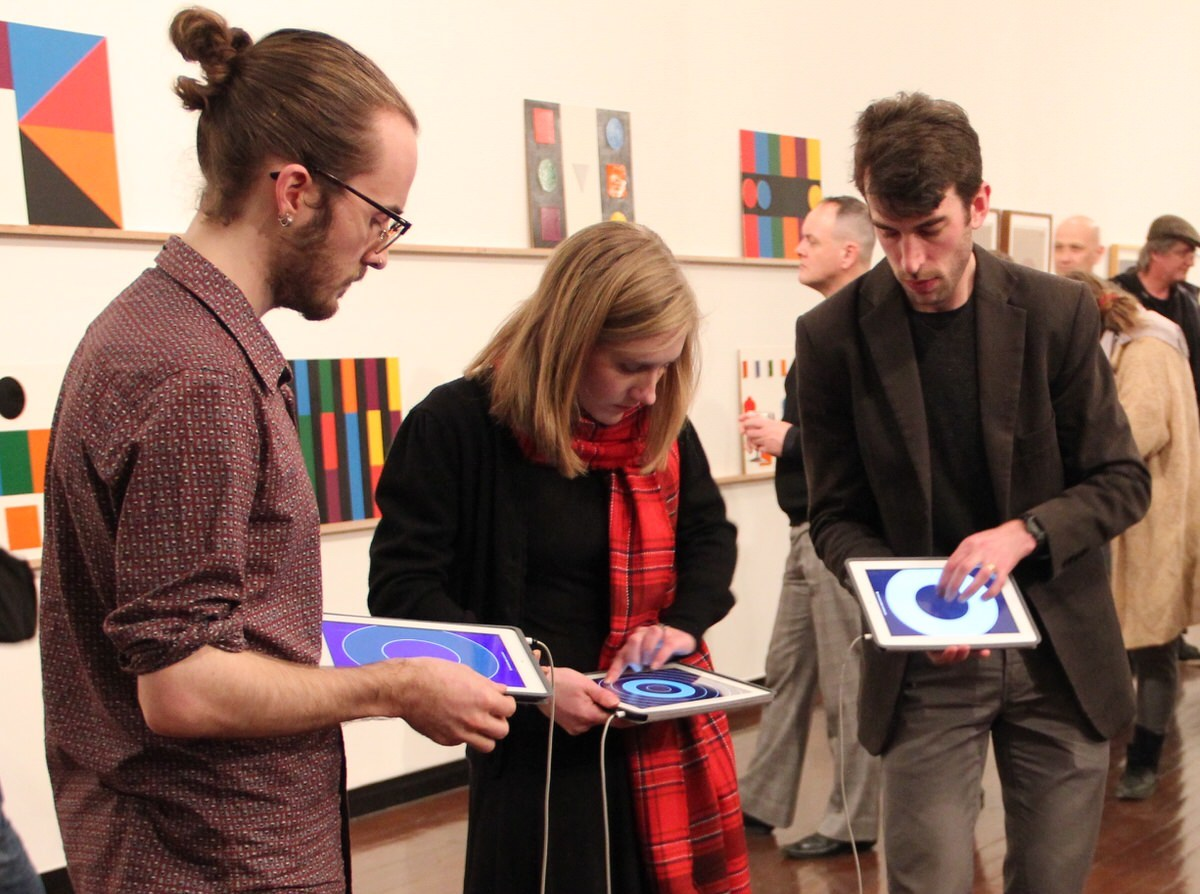
\includegraphics[width=\marginparwidth]{touch-screen-ensemble}
    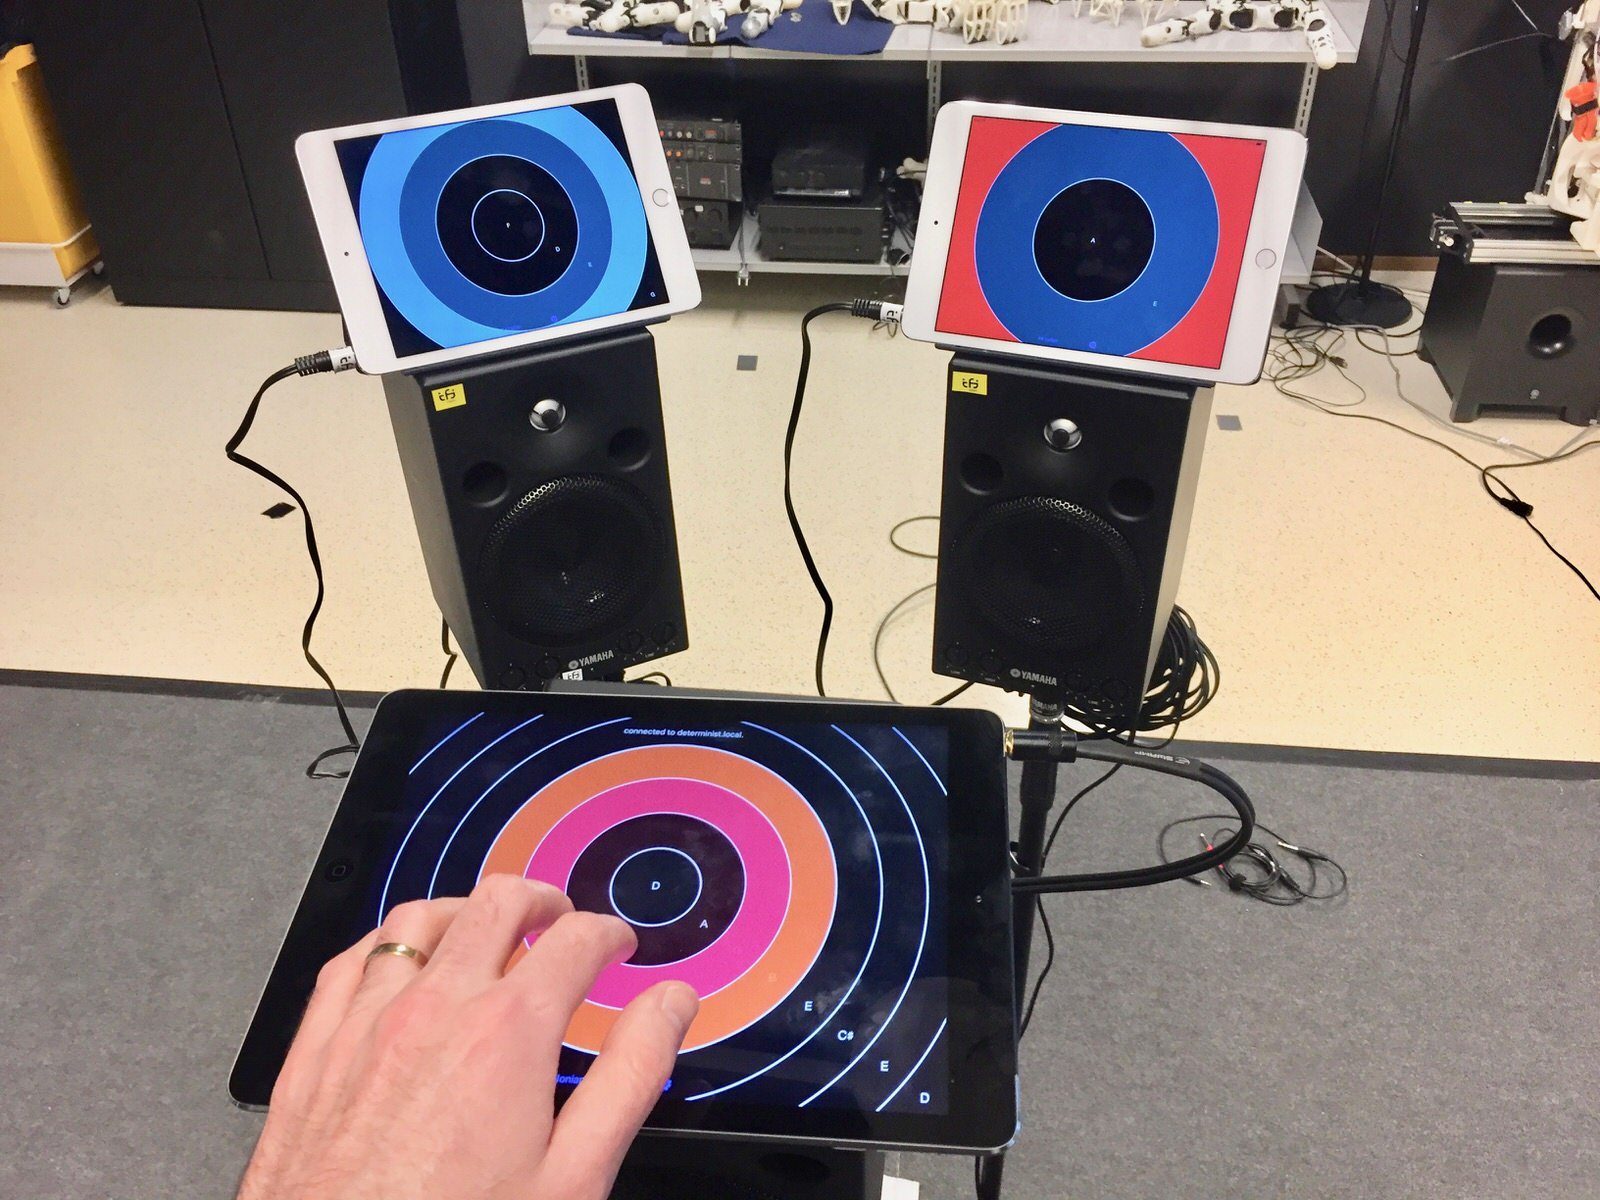
\includegraphics[width=\marginparwidth]{neural-touch-screen-band-small}
    \caption{This system provides an interactive model of an
      improvising touch-screen ensembles (above) using a recurrent neural
      network trained on gestural interaction data. A live performer
      is joined by up to three neural network controlled players (below).}
    \label{fig:system-demo}
\end{marginfigure}

In this work an LSTM-RNN model is used to predict the possible
reactions of free-improvising performers in an ensemble of
touch-screen musicians. Powerful touch-screen devices have enabled
many creative NIME designs~\cite{Gaye:2006qy}. Of particular interest
is how these portable devices can be used in new kinds of ensemble,
such as mobile phone orchestra~\cite{Wang:2014cs}, home-made mobile
device marching bands~\cite{Snyder:2014dp}, and distributed and
participatory mobile gamelan~\cite{Greg-Schiemer:2007mz}. Of the many
affordances of mobile devices\cite{Tanaka:2010sp}, these groups have
explored performance with sound, movement, and light sensors, as well
as their expressive multi-touch displays.

In previous research, a dataset has been collected of more than 150
collaborative performances on touch-screens~\cite{Martin:2016rm}, in
configurations from duets to septets and including a large number of
free-improvised performances. This dataset included time series of raw
touch-data as well as high level touch-gesture interpretations. This
work presents an LSTM-RNN model of ensemble interactions that focuses
on high-level touch gestures.

In this work, a live interaction systems allows a human performer to
lead an RNN-driven ensemble. The performer operates one mobile device
while up to three others are operated by our neural ensemble system.
The gestures of the ensemble are sampled from the output of the RNN
and a touch-synthesis system streams corresponding touch signals to
the other iPads. This system not only applies an RNN to the novel task
of representing ensemble interaction among touch-screen performers,
but allows users to evaluate the quality and utility of the model
directly and to compare the results of different training strategies
through live interaction.

\subsection{Gesture-RNN}

Gesture-RNN is an LSTM-RNN model of ensemble interaction, focussed on
high-level gestural data. The performance format for Gesture-RNN are
time-series of gestural states represented by integers. The corpus of
training data that we have used consists of performances where each
performer has nine possible gestural states (including the nothing
state, or no interaction). The RNN is trained to predict the gestures
of an ensemble of performers given input of a single gesture provided
by a lead performer. The ensemble's previous gestures are also given
as a extra input. This arrangement is illustrated in Figure
\ref{fig:gesture-rnn}.

\begin{marginfigure}
    \includegraphics[width=\marginparwidth]{nn-ensemble-training-sidebar}
    \caption{Gesture-RNN takes a lead players' gesture as input, as
      well as the ensembles previous gesture. The output is the
      predicted response of the ensemble.}
    \label{fig:gesture-rnn}
\end{marginfigure}

Gesture-RNN uses a common architecture of three layers of 512 LSTM
cells followed by a fully connected softmax layer as described by
Sturm et al.~\cite{Sturm:2016rz}. We have produced two ensemble models
using the corpus of gestural data corresponding to duets and quartets.
In each case, the networks were trained with minibatches of 64
performance examples each consisting of 120 time-steps. Each of these
examples corresponds to a 2-minute excerpt of a real collaborative
performance. The networks were implemented in TensorFlow and were
trained on an Nvidia GeForce GTX 1080 GPU.

\section{System Description}

\begin{marginfigure}
    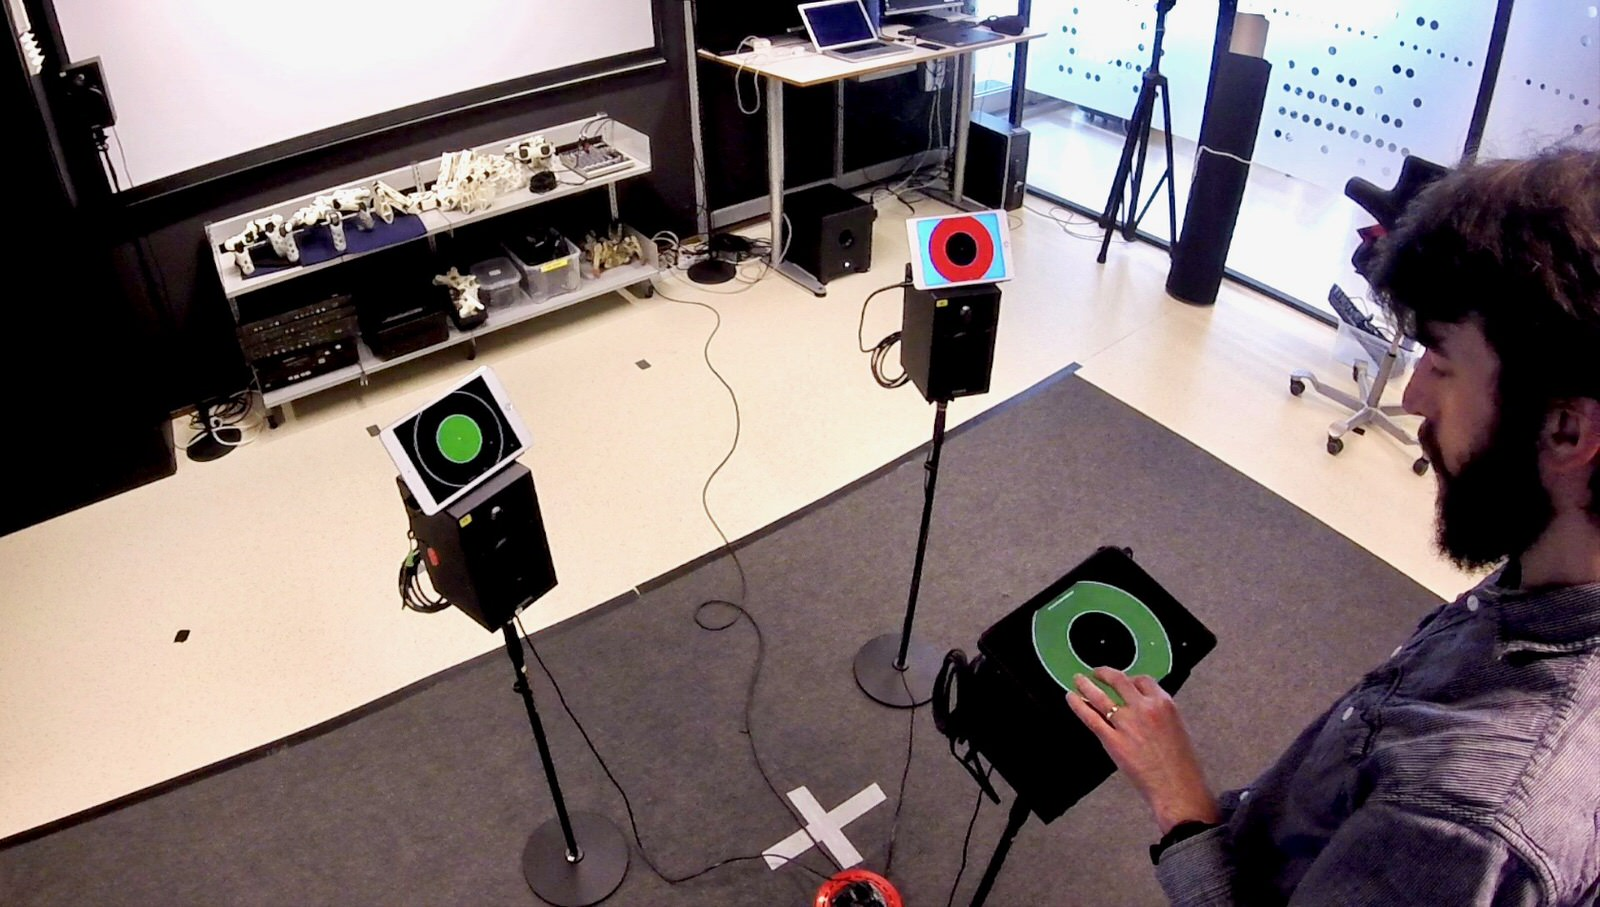
\includegraphics[width=\marginparwidth]{neural-ipad-ensemble-demo-screen}
    \caption{A studio performance with the neural touch-screen
      ensemble. This performance can be found online: \url{https://youtu.be/6eg5VSRqIDA}}
    \label{fig:demo-performance}
\end{marginfigure}

The neural touch-screen ensemble consists of four components: a
touch-screen music app played by the performer and neural ensemble, an
ensemble director agent system, the gesture-RNN, and a touch synthesis
system. The system diagram is shown in
Figure~\ref{fig:live-performance-system}. This system allows a live
performer to interact with the RNN's outputs as if it were a live
group. The iPad app that was used, PhaseRings~\cite{Martin:2016ah},
and ensemble director agent, Metatone Classifier~\cite{Martin:2016xu},
have been explored in previous research but extended here to
incorporate gesture-RNN's quartet model.

During interaction sessions, one performer improvises with the
PhaseRings app. The performer's gestures are classified once every
second by Metatone Classifier. This gesture is used as the lead
performer input for the gesture-RNN. The ensemble inputs for this RNN
are initialised to the nothing gesture at the beginning of the
performance. Output gestures from the RNN are sonified in the
PhaseRings app running on other iPads.

To sonify the outputs of the gesture-RNN, a touch-synthesis system
that streams appropriate touch-data to the ensemble iPads that
corresponds to their generated gesture states. These touch-data are
produced concatenatively from 5-second chunks of touch-data recordings
in the performance corpus. The chunks have been labelled with their
classified gesture and a random chunk is chosen and streamed to each
ensemble iPad every five seconds or whenever a different gestural
state is received from the RNN. The remote-controlled iPads sonify and
visualise this data as if they were being used by a live performer.
Figure \ref{fig:demo-performance} shows a demo performance with this
system that can be viewed online.

\begin{figure}
  \centering
  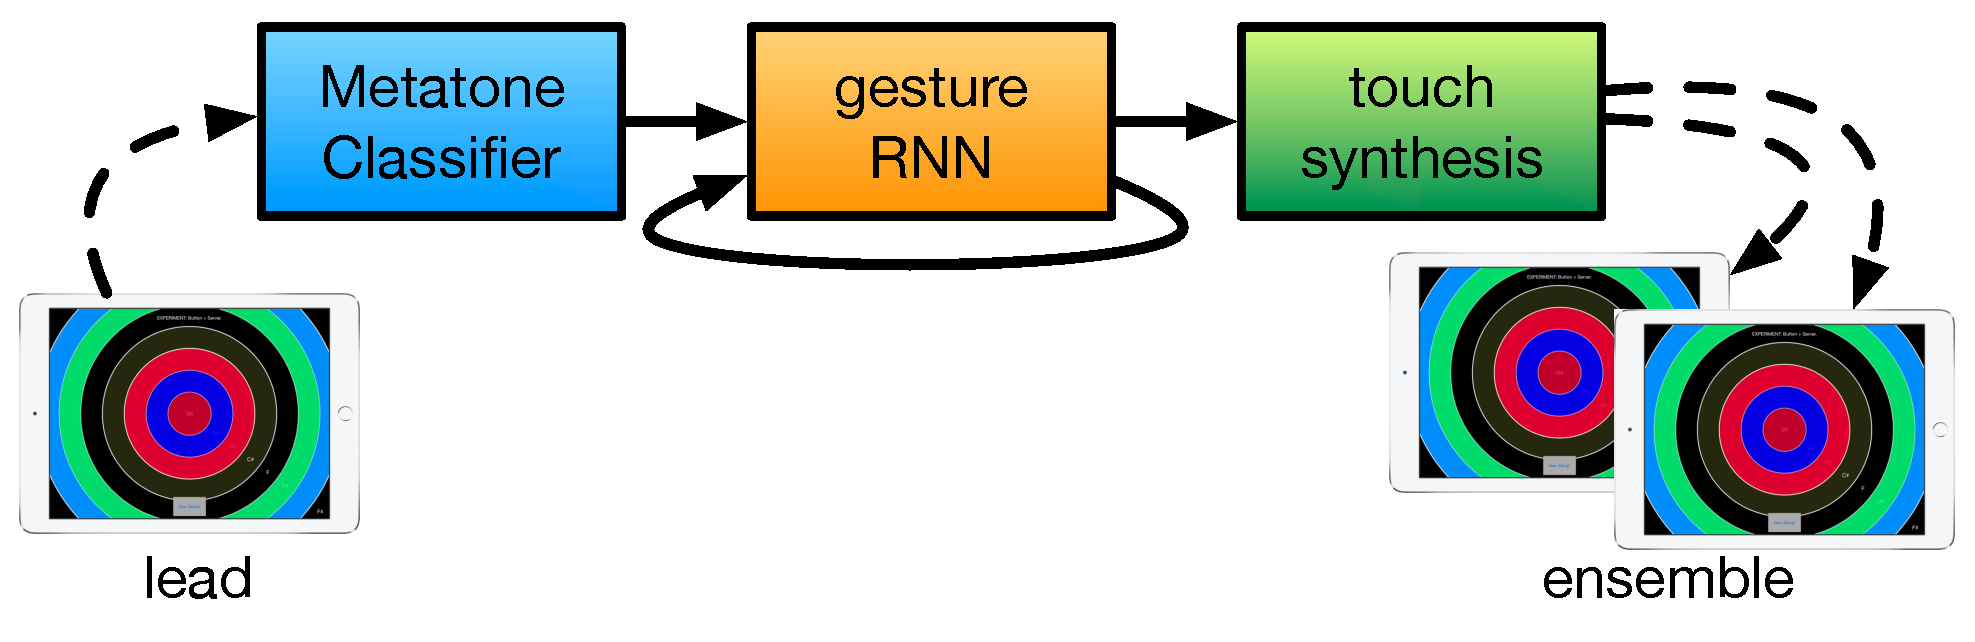
\includegraphics[width=0.7\columnwidth]{live-performance-system}
  \caption{The live performance system classifies gestures from a live
  performer, generates ensemble gestures, then plays back synthesised
  touch events.}\label{fig:live-performance-system}
\end{figure}

\section{Conclusion}

This interactive performance system uses an LSTM-RNN to model ensemble
interactions between touch-screen musicians. It functions as an
interactive neural-network touch-screen ensemble where a single live
performer is accompanied by predicted touch-screen performances of up
to three other band members. Presently, this system is used to
evaluate the creative possibilities of the ensemble interaction model
in real-time. While we have only used the system so far with the
quartet model, it could be used with other RNN designs to explore the
effects of neural network architecture on creative behaviour. It would
also be possible to adapt this system for interaction with other
touch-screen apps, or to include the ensemble responses in the
live-performer's touch-screen interface. Such a system could allow
individual perforemrs to enjoy ensemble-like experiences.

\bibliography{2013ComputerMusic}
\bibliographystyle{ACM-Reference-Format}

\end{document}